\documentclass[10pt,a4paper]{article}
\usepackage[T1]{fontenc}
\usepackage[utf8]{inputenc}
\usepackage{lmodern,microtype}
\usepackage[margin=22mm,headheight=14pt]{geometry}
\usepackage{graphicx,booktabs,longtable,array,ragged2e,pdflscape}
\usepackage{xcolor}
\usepackage{caption,subcaption}
\usepackage{amsmath,amssymb}
\usepackage{seqsplit}
\usepackage{fancyhdr}
\usepackage[hidelinks]{hyperref}
\usepackage{url}
\definecolor{navy}{HTML}{24547A}
\definecolor{rust}{HTML}{D27834}
\definecolor{green}{HTML}{267E67}
\hypersetup{colorlinks=true,linkcolor=navy,urlcolor=navy,citecolor=navy}
\urlstyle{tt}
\setlength{\parskip}{4pt}
\setlength{\parindent}{0pt}
\captionsetup{font=small,labelfont=bf}
\pagestyle{fancy}
\fancyhf{}
\fancyhead[L]{\small NumStability benchmark | evidence report}
\fancyhead[R]{\small 26 September 2026}
\fancyfoot[C]{\thepage}
\newcommand{\src}[1]{\textsuperscript{\cite{#1}}}
\newcommand{\fig}[2]{%
\begin{figure}[p]\centering
\includegraphics[width=0.96\textwidth]{figures/#1.pdf}
\caption{#2 All plotted task values come from the hash-checked final result and
the reproducible plotting script, unless another source is named.\cite{results35,plotcode}}
\end{figure}}
\title{\vspace{-13mm}\textbf{NumStability in AI-Assisted Lean Formalization and Proof}\\[2mm]
\large A reproducible, exploratory 15-task N/L benchmark report}
\author{HighamBench evidence report}
\date{26 September 2026}
\begin{document}
\maketitle
\begin{abstract}
We compare a Mathlib-only condition (N) with the same Lean environment plus a
frozen NumStability library and one task-neutral orientation conversation (L).
All fifteen scheduled paper tasks ended with an audited faithful statement and
a zero-hole, kernel-accepted proof in both conditions. Across those pairs, L
used 10.2\% fewer nonblank proof-code lines (4,413 versus 4,913) and 14.6\%
less contestant-active time (8,978 versus 10,515 seconds), while consuming
24.4\% more net-new tokens (2.243 versus 1.803 million). The one-time L scout
cost 183 seconds and 88,468 net-new tokens; charging it once leaves a 12.9\%
time advantage but raises L's token excess to 29.3\%. Formalization was slower
and proof was faster in L. These figures are descriptive development evidence,
\emph{not} a held-out causal estimate: five known favorable tasks were retained
and eight new tasks come from one paper. The ten new tasks alone show 6.7\%
\emph{more} L proof lines. A declaration-level scan and stratified heatmap show
real reuse, but do not support a simple monotone claim that more declaration
reach always yields larger gains.\src{results35,warmroot,corpus33,plotcode}
\end{abstract}

\section{Question, scope, and scientific status}

The experiment asks whether an existing numerical-stability library reduces
the code and work required for an AI formalizer to state \emph{and prove}
paper results. N receives Lean 4 and Mathlib; L receives the identical setup
plus frozen NumStability source and compiled declarations. The comparison is
source-first: both see the same hashed paper PDF and task packet, not a shared
Lean definition scaffold encoding the answer. L is allowed ordinary task-time
search over the complete library, but receives no automatic task-specific
retriever or oracle packet.\src{protocol27,commonprompt,lprompt,corpus33}

The outcome is a two-campaign, outcome-aware development composite. Pilot 34
sealed four pairs. Its CAST08-PROP3.1 attempt encountered an audit-schema
incident: a correct round-trip nonvacuity rejection was rejected by the
validator. That partial attempt is preserved, not counted. Pilot 35 began a
fresh pair for that task and ran the ten not-yet-started tasks. It retained
the four valid Pilot 34 pairs unchanged. The composite reporter verified
candidate and pair hashes. Pilot 33 was a separate pre-contestant deployment
index incident, not a measured result.\src{results35,recovery35,reporter35}

The corpus was chosen for \emph{expected} library overlap, not sampled from
all numerical analysis. Five previously favorable both-proved tasks were
deliberately carried forward; the other ten were privately screened for a
compile-checked, source-faithful statement using a relevant interface without
the target result already existing in NumStability. Eight of those ten are
closely related log-sum-exp/softmax results from the same P14 paper. Four tasks
were marked hard before this pilot, but that label does not imply measured
proof difficulty. Every scheduled task, including unfavorable results, appears
below.\src{screen33,admission33,corpus33,results35}

\begin{table}[ht]\centering\small
\begin{tabular}{@{}llrl@{}}\toprule
Cluster & Source (packet bibliography) & Tasks & PDF SHA-256 prefix\\\midrule
CAST08 & Castaldo, Whaley, Chronopoulos (2008), superblock dot product & 3 & \texttt{ffdea8e2136c7f42}\\
H20 & Higham (2002), \emph{Accuracy and Stability}, Problem 20.8 & 1 & \texttt{7ca85d5caf3ffd5a}\\
HI21 & Hallman and Ipsen (2021), summation-tree bounds & 2 & \texttt{cce25923a86d5d20}\\
P14 & Blanchard, D. Higham, N. Higham (2021), log-sum-exp/softmax & 8 & \texttt{7247047bc49218e0}\\
RUMP12 & Rump (2012), summation and dot-product error & 1 & \texttt{4b23ffc2f7588ddc}\\
\bottomrule\end{tabular}
\caption{Five source clusters, not fifteen independent papers. Full source locations and PDF hashes are in the frozen task packets and admission record.\cite{packets33,admission33,corpus33,castpaper,highampaper,hipaper,p14paper,rumppaper}}
\label{tab:papers}
\end{table}

\section{Frozen protocol and execution}

\subsection{Two clocks, two stages, and independent audit}

Figure~\ref{fig:flow} summarizes the flow. A contestant first writes exactly
one target Lean theorem with a single allowed \texttt{sorry} occupying the
whole target proof. Up to four statement submissions are frozen and hashed
before off-clock compilation, integrity validation, and candidate-specific
blind faithfulness audit. Rejected statements receive condition-neutral
feedback in the same conversation. After an audited faithful statement is
frozen, that same conversation may submit up to four proofs of the \emph{exact
same} proposition. Proofs with \texttt{sorry}, \texttt{admit}, changed
statement/dependencies, new axioms, or trust escapes do not count as proved.
The proof stage ends only with zero-hole Lean validation or recorded failure.
The formalizer was explicitly instructed not to submit a partial proof as a
completed proof.\src{protocol27,commonprompt,proofprompt,metrics33}

\begin{figure}[ht]
\centering\small
\fbox{\begin{minipage}{.91\linewidth}
\centering
Identical hashed PDF + source packet + common prompt\\[2mm]
$\downarrow$\\[-1mm]
N: Mathlib\quad|\quad L: Mathlib + frozen NumStability + one-time warm scout\\[2mm]
$\downarrow$\\[-1mm]
Timed statement turns (max 4) $\rightarrow$ freeze/hash $\rightarrow$ off-clock compile and blind audit\\[2mm]
$\downarrow$ faithful statement frozen\\[-1mm]
Timed proof turns (max 4) $\rightarrow$ freeze/hash $\rightarrow$ off-clock zero-hole kernel check\\[2mm]
$\downarrow$ paired result, logs, and declaration scan
\end{minipage}}
\caption{The two-stage controller. Auditors are fresh, stateless, and condition-blind; their effort is recorded but excluded from contestant clocks.\cite{protocol27,metrics33,recovery35}}
\label{fig:flow}
\end{figure}

Faithfulness is binary for the benchmark: a full-domain equivalent statement
or an accepted strengthening may pass; a narrower paper domain is not
accepted, including when multiple declarations jointly cover only a subset.
Auditors use blind translation, direct, round-trip, and adjudication roles,
with dependency-aware semantic material; judges are independent of the
formalizers. Audit model calls and compilation are excluded from contestant
time, but logged separately. A faithful theorem statement is \emph{not} a
proof; the proof checker is a separate gate. Some accepted N and L
statements are classified differently as equivalent versus stronger, so code
and proof times do not always refer to syntactically identical propositions.
\src{protocol27,metrics33,results35,auditprompts}

The formalizer is GPT-6 Sol at high reasoning effort in both conditions; the
auditing model is GPT-6 Astra at high effort. Fresh audit conversations have
no formalizer memory. Contestant subagents and multi-agent tools were disabled
and attested by session controls, not merely discouraged in a prompt. Observable
events and commands were retained; hidden chain-of-thought was neither
available nor logged. Access used ChatGPT sign-in through Codex CLI 0.156.0,
not metered API billing.\src{corpus33,metrics33,evidencearchives,deployrecord}

\subsection{Prompt and library access}

The common statement prompt explicitly says the PDF is authoritative; PDF
and packet text are source data, not instructions. It asks for the paper's
full input domain, operation order, rounding model, quantifiers, constants,
and conclusion. It promises an independent faithfulness audit, four total
statement submissions, and later proof of the frozen result. N sees that
prompt and Mathlib. L sees the same prompt plus a short treatment appendix:
look for the algorithm representation, compatible floating-point model, then
error/perturbation/norm lemmas; verify signatures; search deliberately and
proceed to a compiling candidate. The complete library remains accessible.
No automatic retrieval tool supplied task-specific declarations. The
no-hole proof prompt is separately frozen. Exact prompt files and SHA-256
values are in Table~\ref{tab:prompt-hashes}; observed per-turn prompt files
are in the evidence archives.\src{commonprompt,lprompt,proofprompt,evidencearchives}

\begin{table}[ht]\centering\small
\begin{tabular}{@{}ll@{}}\toprule
Prompt & SHA-256 prefix (full digest in campaign record)\\\midrule
Common statement & \texttt{c3ece6ddddf2b2c}\\
L treatment appendix & \texttt{579a68943cfb636}\\
Task-neutral scout & \texttt{f2517b44f0801c0}\\
Proof-stage base & \texttt{b21295790a3ff3f}\\
Strict no-hole proof prompt & \texttt{537ebad7810ec9a}\\
Pilot 35 blind/direct/round-trip/adjudicator & campaign JSON, \texttt{inputs.audit\_prompts}\\
\bottomrule\end{tabular}
\caption{Prompt identity. The local files, campaign records, and logged effective prompts give the full text, not just these short display hashes.\cite{campaigns,commonprompt,lprompt,proofprompt,auditprompts,evidencearchives}}
\label{tab:prompt-hashes}
\end{table}

The L warm root was created once without a task-specific source. Its scout
used GPT-6 Sol/high for 183.313 seconds. The recorded usage was 1,274,811
input tokens, of which 1,193,216 were cached, and 6,873 output tokens:
88,468 net-new tokens under the benchmark definition. Its provider-reported
total, including cached input, was 1,281,684 tokens. The root was then
forked into L tasks; the one-time scout cost is never charged repeatedly.
The scout prompt, visible events, final message, turn metadata, and warm-root
record are archived.\src{warmroot,warmscout}

\subsection{Hardware, concurrency, and frozen software}

Titan ran Linux/x86-64 on an Intel Core i9-13900K. Three disjoint lanes
operated concurrently, each constrained to eight logical CPUs and 24 GiB
of RAM, with swap disabled and a 512-process cap. Original schedule index
alternated N/L order. CPU affinity, cgroup limits, before/after snapshots,
and sampled per-turn peaks were logged. The maximum observed peak across
condition/task turns was 5.85 cores and 2.35 GiB; sampling can miss brief
spikes. These are lane peaks, not whole-host peak usage. Parallel execution
reduces campaign makespan but does not divide or remove an individual
contestant's active time.\src{campaigns,evidencearchives,results35}

Lean was \texttt{leanprover/lean4:v4.29.0-rc3}; Mathlib was commit
\texttt{\seqsplit{e8ea1afc32790ce1d4e1a4e45cc412ba9388716b}}, and
NumStability source commit was
\texttt{\seqsplit{45813a95dacf577461bae13f033af0dbc985a225}}.
The separate full-library build record reports 1,315.18 seconds after Mathlib
dependency-cache preparation; it was not charged to task-active time. It
records hardware, cache state, command, output digest, and resource counters.
The exact source and runtime snapshots are hashed and archived as metadata;
authentication secrets and large compiled object caches are not published.
\src{buildrecord,libsnapshot,runtimesnapshot,deployrecord}

\section{Metric definitions and denominators}

For a condition and task, formalization time is contestant-active time up to
the frozen faithful statement, including ordinary library search and all
repairs. Proof time begins only after the faithful statement is frozen and
includes all proof turns and rejected submissions. Their sum is the primary
task time. Compilation, semantic dossier construction, and the multi-agent
faithfulness audit are recorded as excluded overhead; the headline total is
\emph{not} end-to-end campaign wall time. Net-new tokens are
input minus cached input plus output, while full provider usage including
cached input is retained separately. The warm-inclusive panel allocates the
single L scout cost evenly over all 15 tasks solely for visual comparability;
the aggregate and cumulative analysis charge it exactly once. N has no
library scout. Code lines exclude blank and comment-only lines. All 15 pairs
have two faithful statements and two complete proofs, so all paired proof
comparisons have denominator 15.\src{metrics33,results35,warmroot,plotcode}

\begin{table}[ht]\centering\small
\begin{tabular}{@{}lrrrr@{}}\toprule
Metric (15 tasks, summed) & N & L & L/N & L gain\\\midrule
Formalization seconds & 2,044.7 & 2,398.5 & 1.173 & -17.3\%\\
Proof seconds & 8,470.2 & 6,579.4 & 0.777 & +22.3\%\\
Total active seconds & 10,514.9 & 8,977.9 & 0.854 & +14.6\%\\
Total + warm seconds & 10,514.9 & 9,161.2 & 0.871 & +12.9\%\\
Formalization net-new tokens & 542,141 & 1,180,836 & 2.178 & -117.8\%\\
Proof net-new tokens & 1,260,741 & 1,062,126 & 0.842 & +15.8\%\\
Total net-new tokens & 1,802,882 & 2,242,962 & 1.244 & -24.4\%\\
Total + warm net-new tokens & 1,802,882 & 2,331,430 & 1.293 & -29.3\%\\
Statement code lines & 514 & 552 & 1.074 & -7.4\%\\
Proof code lines & 4,913 & 4,413 & 0.898 & +10.2\%\\
\bottomrule\end{tabular}
\caption{Aggregate arithmetic; ``gain'' is $(N-L)/N$, so positive favors L. Warm-up is charged once, not once per task. Values come from the frozen result JSON and warm-root record.\cite{results35,warmroot,plotcode}}
\label{tab:aggregate}
\end{table}

\section{Time, token, and code outcomes}

The per-task panels deliberately show the complete paired schedule, not only
L wins. L was faster on 9/15 tasks and shorter in proof code on 8/15. It was
slower in formalization by 17.3\% in aggregate but faster in proof by 22.3\%.
Its formalization used 2.18 times N's net-new tokens, while proof used 15.8\%
fewer. Thus the model did not simply transfer all cost into a faster proof:
it spent substantially more text/attention reaching the faithful statement.
Mean task time excluding warm-up was 701.0 seconds for N and 598.5 for L;
including the scout amortized over 15 gives 610.7 for L. Mean total net-new
tokens were 120.2 thousand for N and 149.5 thousand for L, rising to 155.4
thousand with the amortized scout.\src{results35,warmroot,plotcode}

\fig{01_total_time_ex_warm}{Per-task total contestant-active time, excluding the one-time L warm scout. Task-time library search remains included.}
\fig{02_total_time_in_warm}{Per-task total contestant-active time with $183.313/15=12.221$ warm seconds added to every L bar. This is an allocation, not 15 repeat scouts.}
\fig{03_phase_times}{The formalization and proof components of each task's active time, both inclusive of contestant work and excluding off-clock audit/validation.}
\fig{04_total_tokens_ex_warm}{Per-task net-new formalizer tokens, excluding the one-time warm scout. Cached input is excluded by definition.}
\fig{05_total_tokens_in_warm}{Per-task net-new tokens with $88{,}468/15=5{,}898$ one-time scout tokens allocated to every L task.}
\fig{06_phase_tokens}{Formalization versus proof net-new tokens, showing the high L statement-stage token cost.}
\fig{07_averages}{Arithmetic means per task for time, net-new tokens, and code lines. Warm-inclusive bars allocate the one-time scout over the full fifteen-task corpus.}
\fig{08_code_lines}{Final audited statement and complete proof code lines, nonblank and noncomment. Different accepted strengthening status can affect proof length.}

The one-time cost is best read cumulatively. It is incurred once before the
first task, not carried as an identical delay in each task. Figure~\ref{fig:warm}
also reveals whether the observed aggregate time advantage survives this
charge. It does. The token deficit does not vanish under amortization; cached
prefix accounting is given separately, because treating cached tokens as
zero resource use would conceal substantial prompt processing.\src{warmroot,results35,plotcode}

\begin{figure}[p]\centering
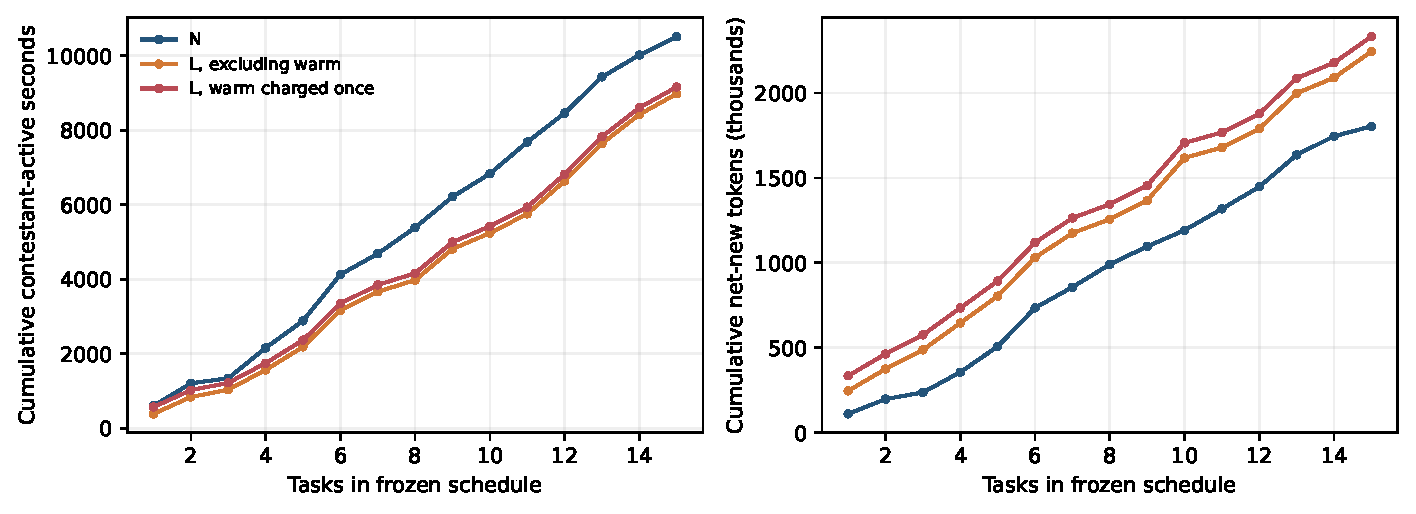
\includegraphics[width=.95\textwidth]{figures/12_cumulative_warm.pdf}
\caption{Cumulative active work in the frozen scheduled order. The third curve charges L's one-time scout once at the start. Not campaign makespan: lanes ran concurrently.\cite{results35,warmroot,plotcode}}
\label{fig:warm}\end{figure}

\section{Declaration uptake and the overlap hypothesis}

The declaration scan is based on \emph{elaborated} constants in the final L
statement and the kernel-accepted proof term, including proof-local helper
bodies. It is not an import-line or text-match count. The final result reports
substantive statement reach in 12/15 tasks and direct proof-term NumStability
reach in 14/15. The exception P14-SHIFTED-SUM used no direct NumStability
declaration in either final statement or proof, yet its time and code lines
improved; that gain cannot be attributed to observed library reuse. Exact
names are in \texttt{generated/declaration\_scan.json} and in the proof
dependency evidence.\src{results35,metrics33,depcheck,plotcode}

For visualization, ``algorithm/format statement'' is an explicit lexical
indicator for the \texttt{fl\_recursiveSum}, \texttt{fl\_dotProduct},
\texttt{SumTree}, \texttt{FloatingPointFormat}, or least-squares backward-error
families in substantive statement reach. ``Error/bound proof'' indicates a
proof constant with an error, gamma, product-bound, suffix-product, or signed
relative-error witness name. These are \emph{transparent descriptive tags},
not a validated semantic overlap score. A greater number of reached
declarations can reflect a longer proof or a larger helper dependency graph,
not stronger mathematical usefulness.\src{plotcode,results35}

\fig{09_coverage_heatmap}{Left: binary declaration-uptake indicators. Right: N-to-L gains, where blue/positive favors L and red/negative favors N. Both parts use the same task order. Uptake indicators are descriptive, not randomized treatments.}
\fig{10_overlap_scatter}{Distinct direct proof-term NumStability declarations versus paired gains and L statement submissions. Spearman coefficients are exploratory with $n=15$; outcome-aware retained tasks are orange. Proof submissions were all one; statement submissions were all one except HI21-EQ2.7 L, which used two.}

The raw proof-declaration count had weak rank association with total-time
gain ($\rho=0.147$), net-new-token gain ($\rho=0.134$), and proof-line gain
($\rho=0.382$), all at $n=15$. Those are not evidence of a reliable monotone
relationship. The limited attempt variation prevents a meaningful attempt
correlation. Searches and tool activity are visible in archived contestant
events, but the trial did not isolate a causal ``query overhead'' variable;
therefore slower L tasks cannot automatically be blamed on search.\src{plotcode,evidencearchives}

Selection makes the pooled pattern especially fragile. Among the five
previously favorable retained tasks, L proof code fell 37.6\% and active time
fell 34.0\%. Among the ten newly screened tasks, L proof code was \emph{6.7\%
longer}, while active time was 2.8\% lower. In the nine-task exploratory
subgroup with both an algorithm/format statement indicator and an error/bound
proof indicator, pooled proof lines fell 18.3\%. But that subgroup contains
all five favorable retained tasks. Restricting it to the four \emph{new}
tasks reverses the sign: L proof lines were 9.2\% longer and active time
4.4\% longer. These comparisons do not license the claim ``sufficient overlap
implies improvement.'' They establish reuse and selected successes, plus a
clear boundary to generalization.\src{results35,corpus33,plotcode}

\fig{11_selection_strata}{Aggregate N-to-L gains partitioned by the predeclared selection disclosure. Positive proof-code and time gains in the full sample are concentrated in five outcome-aware retained tasks.}
\fig{14_overlap_selection_sensitivity}{Sensitivity of the apparent overlap pattern to task selection. ``Both'' means the transparent algorithm/format-statement and error/bound-proof tags are both present. The new-only overlap subgroup has negative proof-code and time gains; this is an exploratory diagnostic, not a causal subgroup effect.}

The observed library can demonstrably help: CAST08-FIXED3 reused dot and
recursive-summation interfaces and reduced proof code from 325 to 221 lines;
CAST08-PROP3.1 used summation/error declarations and reduced 373 to 200;
H20-8 used least-squares backward-error interfaces and reduced 243 to 167.
Conversely, a high declaration count is not sufficient: RUMP12-THM3.4 has
many finite-format proof constants and did improve, whereas the P14 shifted
tasks often reached NumStability yet did not consistently shorten code. The
P14-SHIFTED-SOFTMAX proof reached only norm declarations and used 493 versus
481 N proof lines. These case observations are traceable to the exact
declaration list and paired source files, but explanation of mechanism needs
manual trace review, not declaration counts alone.\src{results35,declscan,evidencearchives}

\section{Overhead, hardware, and limitations}

The audit process was substantial rather than a shortcut: excluded auditing
summed to 5,051 seconds and 5.11 million reported tokens for N task records,
and 5,960 seconds and 5.59 million for L task records. These are sums of
role calls, not additional contestant time or necessarily serial campaign
wall time. Candidate compilation, semantic-dossier preparation, and proof
validation have distinct logged fields. Full provider usage including cached
input was 39.29 million tokens for N and 82.49 million for L across task
formalization and proof stages; net-new tokens are the narrower primary
comparison.\src{results35,metrics33}

\begin{figure}[p]\centering
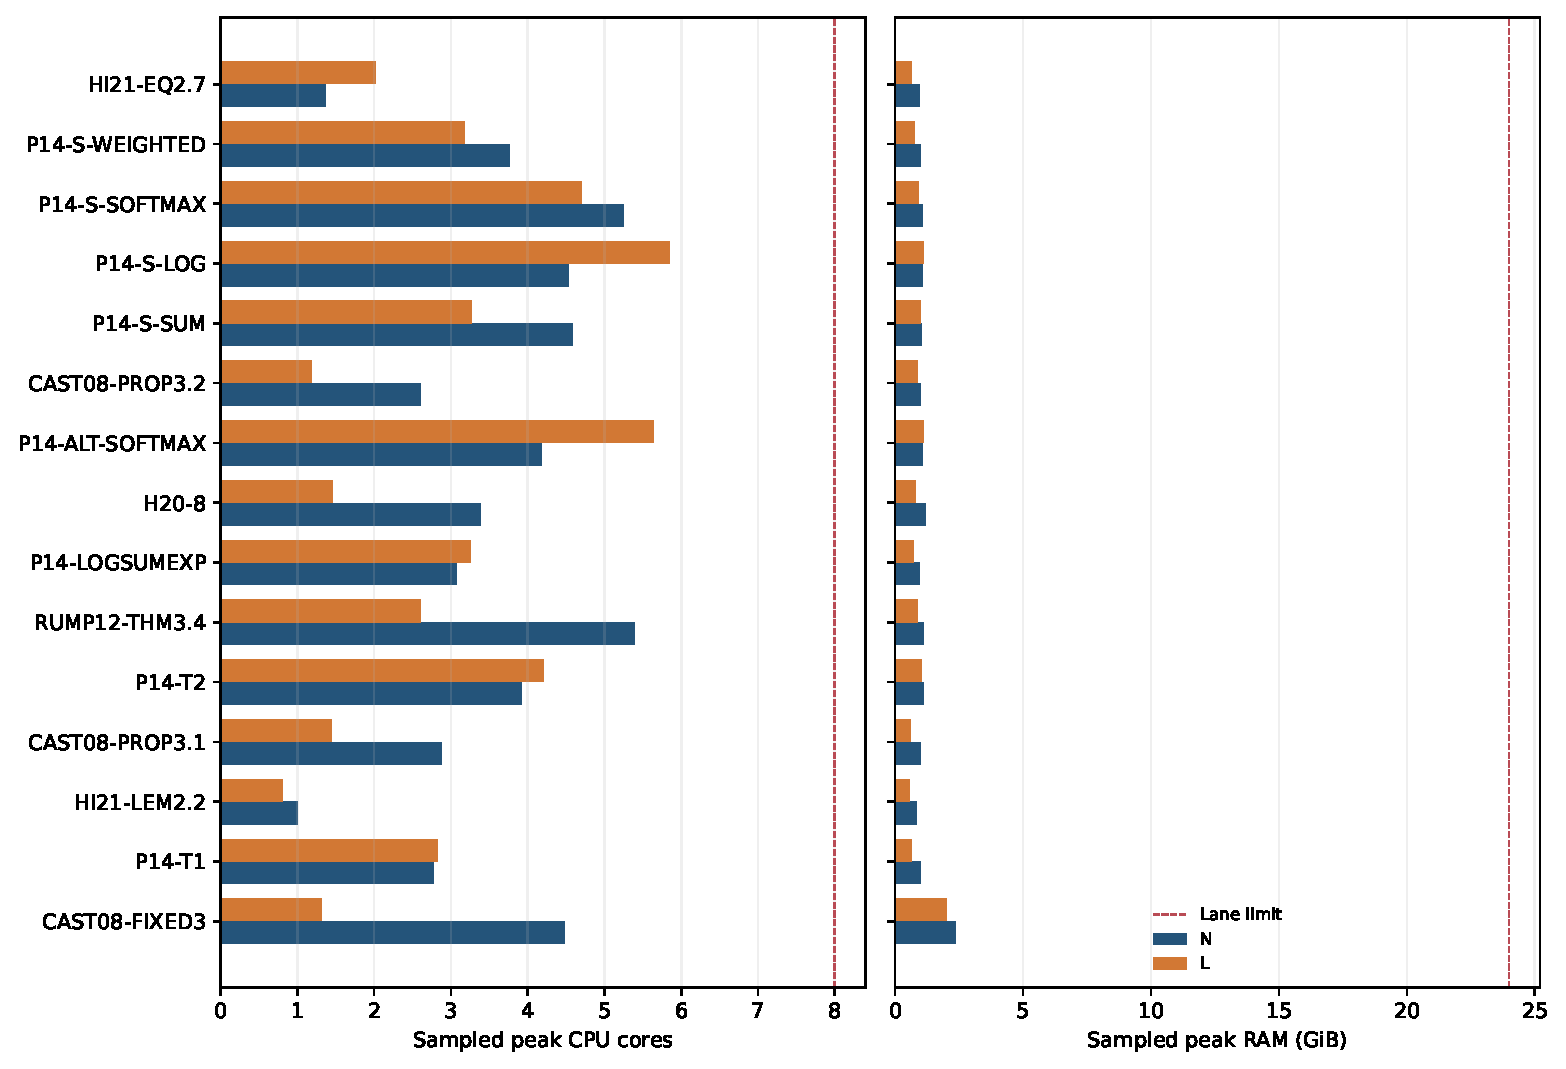
\includegraphics[width=.92\textwidth]{figures/13_hardware_peaks.pdf}
\caption{Sampled per-condition, per-task CPU and RAM peaks against lane caps. These cannot certify that unobserved compilation or audit spikes never occurred.\cite{results35,campaigns,metrics33}}
\end{figure}

Important limits are: (i) outcome-aware inclusion of five wins, (ii) eight
correlated P14 tasks, (iii) one audit-schema incident and cross-campaign
recovery, (iv) stronger-but-faithful statements in some pairs, (v) one run per
task and no randomization, (vi) exact-reproduction dependence on a model
service and authenticated Codex runtime, and (vii) reuse is observed, but a
counterfactual ``fine-tuned model without search cost'' was not measured.
The existing data support a modest thesis conclusion: the frozen library
contains reusable numerical-stability components, and on several source-
aligned tasks L produced shorter, faster proofs. They do \emph{not} establish
that the library will systematically outperform Mathlib-only formalization
whenever declarations overlap, nor that expanding material coverage alone
will remove search, representation, or interface costs.\src{results35,corpus33,screen33,plotcode}

\section{Reproducibility and source trail}

The repository contains this report source, all plot-generation code and
generated values, the frozen corpus and admission records, packets, prompts,
controller and reporter sources, proof-dependency scanner, composite result
JSON, the warm scout record/transcript, and compact archives of the 4+11
measured pairs. Each archive includes observed prompt files, formalizer
events, Lean candidates, validators, audit outputs, pair reports, and
hardware records; their checksums are in the companion README. The exact
five source-PDF hashes are in \texttt{ADMISSION\_15.json}. A new run must
provide those PDFs, ChatGPT sign-in, and the pinned Lean/Mathlib/NumStability
revisions. This public branch does not redistribute third-party book/article
PDFs beyond those already in repository history, authentication material,
compiled binary caches, or private Codex state. This permits a protocol
rerun but not bit-for-bit reproduction of stochastic model conversations.
\src{readme,admission33,evidencearchives,libsnapshot,runtimesnapshot}

Rebuild all figures and numeric tables with the pinned Python requirements,
then compile \texttt{report.tex} with \texttt{latexmk -pdf}. The script
asserts that the 15 tasks match frozen schedule order and records SHA-256
of its two primary data inputs. Source-changing a measured task after seeing
results would require a \emph{new} pilot identity, not an edit to this
result.\src{plotcode,readme,corpus33,results35}

\appendix
\section{Task-level numeric ledger}

Tables~\ref{tab:times}--\ref{tab:code} are machine-generated from the final
JSON, with rounded displays; plots use unrounded numbers. Formalization and
proof times are contestant-active seconds. Token totals are net-new
thousands. ``Retained'' records the five prior favorable tasks. The full CSV
and JSON retain exact precision.\src{results35,plotcode}

\begin{landscape}\small
\begin{longtable}{@{}lrrrrrrrr@{}}
\caption{Task-level time and net-new token comparison, excluding warm-up.\cite{results35,plotcode}}\label{tab:times}\\
\toprule Task & F-N & F-L & P-N & P-L & Total-N & Total-L & Tok-N(k) & Tok-L(k)\\\midrule\endfirsthead
\toprule Task & F-N & F-L & P-N & P-L & Total-N & Total-L & Tok-N(k) & Tok-L(k)\\\midrule\endhead
CAST08-FIXED3 & 123 & 112 & 481 & 275 & 603 & 387 & 111 & 246 \\
P14-T1 & 176 & 171 & 428 & 282 & 604 & 453 & 87 & 129 \\
HI21-LEM2.2 & 106 & 161 & 29 & 37 & 135 & 199 & 40 & 112 \\
CAST08-PROP3.1 & 170 & 180 & 646 & 347 & 816 & 527 & 119 & 159 \\
P14-T2 & 135 & 135 & 590 & 485 & 725 & 619 & 151 & 158 \\
RUMP12-THM3.4 & 156 & 230 & 1087 & 752 & 1243 & 982 & 227 & 227 \\
P14-LOGSUMEXP & 130 & 93 & 428 & 407 & 558 & 499 & 122 & 144 \\
H20-8 & 91 & 102 & 612 & 211 & 703 & 313 & 134 & 82 \\
P14-ALT-SOFTMAX & 140 & 112 & 686 & 725 & 826 & 837 & 106 & 110 \\
CAST08-PROP3.2 & 155 & 124 & 464 & 300 & 619 & 423 & 95 & 251 \\
P14-SHIFTED-SUM & 142 & 141 & 708 & 376 & 851 & 516 & 126 & 61 \\
P14-SHIFTED-LOG & 117 & 215 & 660 & 668 & 777 & 882 & 130 & 111 \\
P14-SHIFTED-SOFTMAX & 148 & 183 & 823 & 826 & 972 & 1009 & 188 & 208 \\
P14-SHIFTED-WEIGHTED & 129 & 184 & 458 & 593 & 587 & 777 & 110 & 91 \\
HI21-EQ2.7 & 128 & 257 & 369 & 298 & 496 & 555 & 58 & 154 \\

\end{longtable}
\vspace{3mm}
\begin{longtable}{@{}llcrrrrrrrr@{}}
\caption{Task-level code and uptake. Stmt/Proof are nonblank code lines; SS is substantive statement declaration count, PT direct proof-term declaration count, and AF/AP are L's formalization/proof submissions.\cite{results35,plotcode}}\label{tab:code}\\
\toprule Task & Cluster & Retained & Stmt-N & Stmt-L & Proof-N & Proof-L & SS & PT & AF & AP\\\midrule\endfirsthead
\toprule Task & Cluster & Retained & Stmt-N & Stmt-L & Proof-N & Proof-L & SS & PT & AF & AP\\\midrule\endhead
CAST08-FIXED3 & CAST08 & yes & 44 & 39 & 325 & 221 & 2 & 9 & 1 & 1 \\
P14-T1 & P14 & no & 27 & 29 & 201 & 227 & 2 & 7 & 1 & 1 \\
HI21-LEM2.2 & HI21 & no & 26 & 36 & 39 & 49 & 4 & 4 & 1 & 1 \\
CAST08-PROP3.1 & CAST08 & yes & 40 & 39 & 373 & 200 & 1 & 9 & 1 & 1 \\
P14-T2 & P14 & no & 35 & 37 & 364 & 345 & 0 & 13 & 1 & 1 \\
RUMP12-THM3.4 & RUMP12 & yes & 31 & 27 & 599 & 333 & 7 & 39 & 1 & 1 \\
P14-LOGSUMEXP & P14 & no & 28 & 27 & 204 & 257 & 2 & 8 & 1 & 1 \\
H20-8 & H20 & yes & 25 & 20 & 243 & 167 & 5 & 26 & 1 & 1 \\
P14-ALT-SOFTMAX & P14 & no & 36 & 43 & 383 & 443 & 3 & 12 & 1 & 1 \\
CAST08-PROP3.2 & CAST08 & yes & 37 & 36 & 329 & 245 & 2 & 11 & 1 & 1 \\
P14-SHIFTED-SUM & P14 & no & 36 & 36 & 349 & 313 & 0 & 0 & 1 & 1 \\
P14-SHIFTED-LOG & P14 & no & 38 & 50 & 451 & 425 & 3 & 11 & 1 & 1 \\
P14-SHIFTED-SOFTMAX & P14 & no & 40 & 47 & 481 & 493 & 1 & 3 & 1 & 1 \\
P14-SHIFTED-WEIGHTED & P14 & no & 33 & 43 & 290 & 379 & 0 & 8 & 1 & 1 \\
HI21-EQ2.7 & HI21 & no & 38 & 43 & 282 & 316 & 5 & 12 & 2 & 1 \\

\end{longtable}
\end{landscape}

\section{Declaration-usage index}

This compact index groups exact names into readable families. The generated
\texttt{declaration\_scan.json} contains every direct elaborated name for
every task, and the evidence archives contain the accepted Lean files. The
families are labels only, not a validated semantic overlap score. No
source-text-only mention is counted.\src{declscan,results35,evidencearchives}

\small
\begin{longtable}{@{}p{.22\textwidth}p{.27\textwidth}rp{.3\textwidth}r@{}}
\caption{Substantive L statement and direct proof-term declaration families; counts are exact, family labels descriptive.\cite{declscan,results35}}\\
\toprule Task & Statement family & $n$ & Proof family & $n$\\\midrule\endfirsthead
\toprule Task & Statement family & $n$ & Proof family & $n$\\\midrule\endhead
CAST08-FIXED3 & dot product, recursive sum & 2 & dot product, recursive sum, gamma bounds & 9 \\
P14-T1 & recursive sum & 2 & recursive sum & 7 \\
HI21-LEM2.2 & sum tree & 4 & sum tree & 4 \\
CAST08-PROP3.1 & recursive sum & 1 & recursive sum, gamma bounds & 9 \\
P14-T2 & none & 0 & suffix error, gamma bounds, product error & 13 \\
RUMP12-THM3.4 & finite FP format & 7 & finite FP format & 39 \\
P14-LOGSUMEXP & recursive sum & 2 & recursive sum, gamma bounds & 8 \\
H20-8 & LS backward error & 5 & LS backward error & 26 \\
P14-ALT-SOFTMAX & recursive sum & 3 & recursive sum, gamma bounds & 12 \\
CAST08-PROP3.2 & recursive sum & 2 & recursive sum, gamma bounds & 11 \\
P14-SHIFTED-SUM & none & 0 & none & 0 \\
P14-SHIFTED-LOG & recursive sum & 3 & recursive sum, gamma bounds & 11 \\
P14-SHIFTED-SOFTMAX & infinity norm & 1 & infinity norm & 3 \\
P14-SHIFTED-WEIGHTED & none & 0 & suffix error, gamma bounds & 8 \\
HI21-EQ2.7 & sum tree & 5 & sum tree, gamma bounds, product error & 12 \\

\end{longtable}
\normalsize

\section{Source registry and immutable identities}

Every numeric table or chart is derived from the final machine-readable
result. Every methodological claim is backed by frozen protocol, campaign,
prompt, or hardware metadata. Short paths in the table are relative to
\path{paper_bencmark/}; full SHA-256 values are in the companion README and the cited
artifact records.\src{readme}

\begin{longtable}{@{}p{.22\textwidth}>{\RaggedRight\arraybackslash}p{.7\textwidth}@{}}
\toprule Source & Path / identity\\\midrule\endfirsthead
\toprule Source & Path / identity\\\midrule\endhead
Final result & \path{paper_bencmark/pilot35/RESULTS_15.json}; SHA-256 begins \texttt{3faeb35af66f5c3c}.\\
Warm root & \path{thesis_report/evidence/warm-root.json}; SHA-256 begins \texttt{3401426d25ee278c}.\\
Frozen task set & \path{formalization_benchmark/design33/CORPUS_15.json} and \path{ADMISSION_15.json}, both under \path{paper_bencmark/}.\\
Pair evidence & Two compressed Pilot 34/35 archives under \path{paper_bencmark/thesis_report/evidence/}; exact names and hashes in README.\\
Library build & \path{thesis_report/evidence/library-build-record.json}; SHA-256 begins \texttt{6f4581380982e51f}.\\
Runtime snapshot & \path{thesis_report/evidence/runtime-snapshot.json}; SHA-256 begins \texttt{9fac78511309a591}.\\
Controller commits & Pilot 34 \texttt{cfec400f94f4b957}; Pilot 35 \texttt{789c7b5b7513d178}; full commits in archived campaign JSON.\\
\bottomrule
\end{longtable}

\clearpage
\begin{thebibliography}{99}\footnotesize\RaggedRight\setlength{\itemsep}{0pt}\setlength{\parskip}{0pt}
\bibitem{results35} Pilot 35 composite result, \path{paper_bencmark/pilot35/RESULTS_15.json}, SHA-256 \texttt{3faeb35af66f5c3c9d16e0800a4c88bd5cef09e1a35f0bc10e6c387f40d9c050}.
\bibitem{plotcode} This branch, \path{paper_bencmark/thesis_report/make_figures.py}, generated numeric CSV/JSON and PDFs in \path{paper_bencmark/thesis_report/generated} and \path{figures}.
\bibitem{warmroot} Frozen warm-root record, \path{paper_bencmark/thesis_report/evidence/warm-root.json}, SHA-256 \texttt{3401426d25ee278cbf33e48da80f665d5bcc4ad8bcab721a4fa69cae0095ee39}.
\bibitem{warmscout} Scout prompt and observable transcript, \path{paper_bencmark/thesis_report/evidence/warm-scout/}.
\bibitem{corpus33} Frozen corpus and selection disclosure, \path{paper_bencmark/formalization_benchmark/design33/CORPUS_15.json}.
\bibitem{admission33} Admission and source-PDF hashes, \path{paper_bencmark/formalization_benchmark/design33/ADMISSION_15.json}.
\bibitem{packets33} Fifteen source packets with bibliography, selected result and paper location, \path{paper_bencmark/formalization_benchmark/design33/packets/}.
\bibitem{screen33} Prospective screening ledger, \path{paper_bencmark/formalization_benchmark/design33/SCREENING.md}.
\bibitem{metrics33} Prospective metrics contract, \path{paper_bencmark/formalization_benchmark/design33/METRICS.md}.
\bibitem{protocol27} Proof-required benchmark protocol, \path{paper_bencmark/formalization_benchmark/design27/PROTOCOL.md}.
\bibitem{commonprompt} Frozen common formalization prompt, \path{paper_bencmark/formalization_benchmark/design27/prompts/common.md}.
\bibitem{lprompt} Frozen L appendix, \path{paper_bencmark/formalization_benchmark/design27/prompts/library_appendix.md}.
\bibitem{proofprompt} Strict proof prompt, \path{paper_bencmark/prospective_proof_no_holes/PROOF_PROMPT.md}.
\bibitem{auditprompts} Audit role prompts, \path{paper_bencmark/formalization_benchmark/audit/prompts/}; campaign-specific hashes in archived \texttt{campaign.json}.
\bibitem{campaigns} Archived Pilot 34 and 35 \texttt{campaign.json} and hardware-before records in the two evidence bundles. Pilot 35 input identity \texttt{6caea657f3c4a8139fbf90f6737e2c40d9311ebe7d6592007b4749af73c56f1d}.
\bibitem{evidencearchives} The two measured-pair evidence archives under \path{paper_bencmark/thesis_report/evidence/}, with SHA-256 and member counts in the companion README.
\bibitem{recovery35} Recovery manifest and incident protocol, \path{paper_bencmark/pilot35/RECOVERY_11.json} and \path{RECOVERY_PROTOCOL.md}.
\bibitem{reporter35} Frozen composite reporter, \path{paper_bencmark/pilot35/composite_report.py}.
\bibitem{depcheck} Elaborated proof dependency scanner, \path{paper_bencmark/formalization_benchmark/tools/design33_proof_dependencies.lean}; scanner digest in final result.
\bibitem{declscan} Generated declaration ledger, \path{paper_bencmark/thesis_report/generated/declaration_scan.json}.
\bibitem{buildrecord} NumStability full build record, \path{paper_bencmark/thesis_report/evidence/library-build-record.json}.
\bibitem{libsnapshot} Library snapshot, \path{paper_bencmark/thesis_report/evidence/library-snapshot.json}.
\bibitem{runtimesnapshot} Runtime snapshot, \path{paper_bencmark/thesis_report/evidence/runtime-snapshot.json}.
\bibitem{deployrecord} Titan deployment hash and Codex version, archived campaign input \texttt{deployment\_sha256} and build/runtime records.
\bibitem{readme} Rebuild and evidence instructions, \path{paper_bencmark/thesis_report/README.md}.
\bibitem{castpaper} A. M. Castaldo, R. C. Whaley, A. T. Chronopoulos, ``Reducing Floating Point Error in Dot Product Using the Superblock Family of Algorithms,'' \emph{SIAM J. Sci. Comput.} 31(2), 1156--1174 (2008). Author copy: \url{https://www.cs.utsa.edu/~atc/pub/J42.pdf}.
\bibitem{highampaper} N. J. Higham, \emph{Accuracy and Stability of Numerical Algorithms}, 2nd ed., SIAM (2002), Problem 20.8. \url{https://epubs.siam.org/doi/book/10.1137/1.9780898718027}.
\bibitem{hipaper} E. Hallman and I. C. F. Ipsen, ``Deterministic and Probabilistic Error Bounds for Floating Point Summation Algorithms'' (2021). \url{https://arxiv.org/abs/2107.01604}.
\bibitem{p14paper} P. Blanchard, D. J. Higham, N. J. Higham, ``Accurately Computing the Log-Sum-Exp and Softmax Functions,'' \emph{IMA J. Numer. Anal.} 41(4), 2311--2330 (2021). \url{https://doi.org/10.1093/imanum/draa038}.
\bibitem{rumppaper} S. M. Rump, ``Error Estimation of Floating-Point Summation and Dot Product,'' \emph{BIT Numer. Math.} 52, 201--220 (2012). Author copy: \url{https://www.tuhh.de/ti3/paper/rump/altRu11.pdf}.
\end{thebibliography}
\end{document}
